\documentclass[conference]{IEEEtran}

%% INFOCOM 2010 addition: 
%\makeatletter
%\def\ps@headings{%
%\def\@oddhead{\mbox{}\scriptsize\rightmark \hfil \thepage}%
%\def\@evenhead{\scriptsize\thepage \hfil \leftmark\mbox{}}%
%\def\@oddfoot{}%
%\def\@evenfoot{}}
%\makeatother
%\pagestyle{headings}

\usepackage{graphicx}
\usepackage{url}

\newcommand{\noteperso}[1]{\begin{center}
 \fbox{\begin{minipage}{6cm}#1\end{minipage}}\end{center}}
%\renewcommand{\noteperso}{}

\newcommand{\ie}{{\em i.e.}}
\newcommand{\eg}{{\em e.g.}}

%\renewcommand{\includegraphics}{}

\newcommand{\ping}{{\tt ping}}
\newcommand{\traceroute}{{\tt traceroute}}
\newcommand{\icmp}{{\sc icmp}}
\newcommand{\echo}{{\sc echo}}
\newcommand{\request}{{\sc request}}
\newcommand{\reply}{{\sc reply}}
\newcommand{\ttl}{{\sc ttl}}
\newcommand{\as}{{\sc as}}
\newcommand{\ip}{{\sc ip}}
\newcommand{\udp}{{\sc udp}}
\newcommand{\bgp}{{\sc bgp}}
\newcommand{\atm}{{\sc atm}}
\newcommand{\mpls}{{\sc mpls}}


%%%%%%%%%%%%%%%%%%%%%%%%%%%%%%%%%%%%%%%%%%%%%%%%%%%%%%%%%%%%%%
%%%%%%%%%%%%  PACKAGES FIGURES  %%%%%%%%%%%%%%%%%%%%%%%%%%%%%%
%%%%%%%%%%%%%%%%%%%%%%%%%%%%%%%%%%%%%%%%%%%%%%%%%%%%%%%%%%%%%%



%\usepackage{pgf}
%\usepackage{xcolor}
%\usepackage{subfigure}
%\usepackage[dvips]{epsfig} % pour les pstex_t
%\usepackage{epic,eepic}
\usepackage{graphicx,color}
%\usepackage{pstcol,pst-fill,pst-grad} % pour les pstex_t


%%%%%%%%%%%%%%%%%%%%%%%%%%%%%%%%%%%%%%%%%%%%%%%%%%%%%%%%%%%%%
%%%%%%%%%%%%%%%%    COMMANDES CHRISTOPHE    %%%%%%%%%%%%%%%%%
%%%%%%%%%%%%%%%%%%%%%%%%%%%%%%%%%%%%%%%%%%%%%%%%%%%%%%%%%%%%%
\newcommand{\comment}[1]{}


\begin{document}

\title{
Rigorous Measurement of IP-level Neighborhood\\
\smallskip
of Internet Core Routers
}


\author{\IEEEauthorblockN{Christophe Crespelle, Matthieu Latapy and \'Elie Rotenberg}
\IEEEauthorblockA{LIP6 -- CNRS and Universit\'e Pierre et Marie Curie -- Paris 6\\
104 avenue du pr\'esident Kennedy, 75016 Paris, France\\
Email: Firstname.Lastname@lip6.fr}
}


%\author{Christophe Crespelle, Matthieu Latapy and \'Elie Rotenberg}

%\institute{LIP6 -- CNRS and Universit\'e Pierre et Marie Curie -- Paris 6\\
%104 avenue du pr\'esident Kennedy, 75016 Paris, France\\
%{\tt Firstname.Lastname@lip6.fr}}


\maketitle

\begin{abstract}
Many contributions use the degree distribution
of IP-level internet topology. However, current knowledge
of this property relies on biased and erroneous
measurements, and so it is subject to much debate.
We introduce here a new approach, dedicated to the core of the internet, which avoids the issues 
raised by classical measurements. It is based on the 
measurement of IP-level neighborhood of internet core
routers, for which we design and implement a rigorous 
method. It consists in sending \traceroute\ probes from 
many monitors distributed in the internet towards a 
given target router and carefully selecting the relevant
information in collected data. Using simulations, we provide
strong evidence of the accuracy of our approach. We then conduct 
real-world measurements illustrating the practical 
effectiveness of our method. This constitutes a significant
step towards reliable knowledge of the IP-level
degree distribution of the core of the internet.
\end{abstract}

%%%%%%%%%%%%%%%%%%%%%%%%%%%%%%%%%%%%%%%%%%%%%%%%%%%%%%%%%%%%%%%
%%%%%%%%%%%%%%%%%%%%%%%%%%%%%%%%%%%%%%%%%%%%%%%%%%%%%%%%%%%%%%%
\section{Introduction}
%%%%%%%%%%%%%%%%%%%%%%%%%%%%%%%%%%%%%%%%%%%%%%%%%%%%%%%%%%%%%%%
%%%%%%%%%%%%%%%%%%%%%%%%%%%%%%%%%%%%%%%%%%%%%%%%%%%%%%%%%%%%%%%
\label{sec-introduction}



{\em "A very general but largely ignored fact about Internet-related measurements is that what we can measure in an internet-like environment is typically not the same as what we really want to measure (or what we think we actually measure)."}\cite{willinger}
This is particularly true for \traceroute\ measurement of the topology. Maps are obtained by merging the paths obtained from a limited number of monitors to many targets. It has been shown that doing so leads to intrinsically biased views \cite{DBLP:conf/infocom/LakhinaBCX03,DBLP:journals/jacm/AchlioptasCKM09,DBLP:journals/tcs/DallAstaABVV06,DBLP:conf/infocom/GuillaumeL05,DBLP:journals/cn/GuillaumeLM06}. The classical assumption is that the bias on observed properties becomes less significant when the sample grows. However, the relevance of this assumption is far from trivial and it was even proved that it is false in some cases at least \cite{DBLP:conf/infocom/LatapyM08}.

In addition, \traceroute\ outputs themselves contain much erroneous information. This may be due to mis-configured routers, route dynamics, or circuit networks. Some of these errors are evidenced and discussed in \cite{willinger,DBLP:conf/sigcomm/SherwoodBS08,DBLP:journals/ton/SpringMWA04,DBLP:journals/cn/VigerACMLFT08,DBLP:conf/imc/AugustinCOVFLMT06}. Correcting such errors is extremely difficult in general, and often impossible. In particular, this is the case of erroneous links induced in \texttt{tarceroute} outputs by load-balancing on the network. The specificity of our approach allows us to tackle this problem.

We explore here a new approach for the measurement of the degree distribution of the IP-level topology of the core of the internet, which is one of its main properties.
This approach does not rely anymore on the collection of a large sample obtained by merging \traceroute\ outputs. Instead, we propose to select internet core routers, rigorously estimate their degrees, and infer the degree distribution from these. The success of this approach relies on our ability to get at least one interface of each IP-level neighbor of the router. Then, using anti-aliasing methods \cite{spring04how,DBLP:conf/imc/BenderSS08,DBLP:conf/sigcomm/SherwoodBS08,DBLP:journals/ton/SpringMWA04}, one may obtain the list of routers in the target neighborhood.
It must be clear that the selection of internet core routers as well as anti-aliasing are non trivial issues. We do not address these problems here, which we consider as future work, and focus on the key point of our measurement approach: obtaining an interface of each neighbor of the target.

\subsection*{Contribution}
We design a rigorous method for the measurement of the neighborhood of internet core routers. We show its validity by simulations, and its practical effectiveness by a sample measurement. We thereby settle an important basis for reliable estimation of the degree distribution of IP-level internet topology, independent of any biased sample and robust to erroneous \traceroute\ information due to load-balancing.


% \marginpar{citer Faloutsos, et Skitter?}


%%%%%%%%%%%%%%%%%%%%%%%%%%%%%%%%%%%%%%%%%%%%%%%%%%%%%%%%%%%%%%%
%%%%%%%%%%%%%%%%%%%%%%%%%%%%%%%%%%%%%%%%%%%%%%%%%%%%%%%%%%%%%%%
\section{Our approach}\label{sec-approach}
%%%%%%%%%%%%%%%%%%%%%%%%%%%%%%%%%%%%%%%%%%%%%%%%%%%%%%%%%%%%%%%
%%%%%%%%%%%%%%%%%%%%%%%%%%%%%%%%%%%%%%%%%%%%%%%%%%%%%%%%%%%%%%%

The classical approach to estimate the degree distribution of IP-level internet topology consists in observing it on a {\em map} of this topology. Such maps are obtained by merging the outputs of many \traceroute\ measurements (each such measurement being supposed to give an IP-level route, and so a path in the corresponding topology). The underlying assumptions are both that errors which may occur in \traceroute\ measurements may be neglected, and that the degree distribution observed on large maps is similar to the actual one. However, the validity of both assumptions is far from established, and many results even seem to show that they are invalid: the measurement method in itself produces biased data \cite{DBLP:conf/infocom/LakhinaBCX03,DBLP:journals/jacm/AchlioptasCKM09,DBLP:journals/tcs/DallAstaABVV06,DBLP:conf/infocom/GuillaumeL05,DBLP:journals/cn/GuillaumeLM06,DBLP:conf/infocom/LatapyM08}, and route dynamics and other internet features lead to many errors in observed routes \cite{willinger,DBLP:conf/sigcomm/SherwoodBS08,DBLP:journals/ton/SpringMWA04,DBLP:journals/cn/VigerACMLFT08,DBLP:conf/imc/AugustinCOVFLMT06}.


The main objective of our approach is to get rid of the issues raised by the map construction. Instead, we focus on the measurement of the strict information needed to observe the property of interest. In our case, we aim at obtaining the exact degree of a given node of the internet. Doing so for many random nodes opens the way to rigorous inference of the actual degree distribution. Clearly, the more nodes we consider, the more precise the inference may be. However, even inference from a relatively small sample would lead to significant improvement of the current situation, if the degrees in the sample are correctly measured.


In addition, our approach reveals other key advantages. First, it clarifies our understanding of the limitations of the measurement process. While \cite{DBLP:conf/imw/BarfordBBC01} argue on the impact of adding sources or destinations in the classical approach, this impact is quite clear with our approach: adding sources increases the precision of our estimation of target degrees, and adding destinations increases the representativity of the sample of nodes used to infer the distribution.

Another benefit of our approach is that the operation of estimation of the degree of a given target, or a set of targets, is atomic: at the end of such an operation, we instantaneously get the desired degrees and we can conduct a new measurement on a different set of destinations. This is not possible with classical measurements which cannot merged only part of the collected \texttt{traceroute} outputs: the result is available only at the end of the measurement, which must last long in order to get a large enough sample of the graph.

With our approach, repeating the atomic measurement operation, we can collect degrees of a set of targets as wide as desired, in order to infer the degree distribution. Moreover, as a round of measurement is short, it is not too sensitive to changes in the network topology. Indeed, these changes artificially increase the degree of affected nodes by making them appear adjacent both to their earlier neighbors and to their newer ones.
On the opposite, because they require long observation periods, classical measurements are quite sensitive to these changes of the topology.
At last, note that the time locality of our atomic measurement operation makes it possible to observe changes in the degree distribution along time, without suffer from changes of the topology.



In order to get the degree of a given router, called {\em target}, we launch \icmp\ \traceroute\ probes\footnote{The choice of \icmp\ was shown to induce less complaints by network administrators, and to have no significant impact on our measurements.}
from many monitors towards this target. The last hop of each traceroute gives in principle an interface (IP address) of an IP-level neighbor of the target. The key objective here is to ensure that we reach the target passing through all of its neighbors. See Figure~\ref{fig-approach} (left).



\begin{figure}
\centering
\input{approach.pstex_t}
\caption{
Left: an example of target $t$ in the core. The routes coming from the set of monitors goes through all of its neighbors.
Right: an example of target $t'$ in the border. Only the neighbor of $t'$ accessible from the core is discovered.
Monitors are represented by blue squares. Nodes in the core are bigger than those in the border. The links of the routes from the monitors to the target are black, while other links are gray.
}
\label{fig-approach}
\end{figure}


Classically, internet IP-level topology is divided into two parts: the \emph{core} and the \emph{border}. The core is defined as the network obtained by removing all trees attached to it ({\em i.e.} iteratively removing all nodes with only one link). The border is the union of these removed trees.
Here, we focus on the degree distribution of the core of the internet. While the tree structure of the border simply carries traffic from end-hosts up to the core and from the core down to end-hosts, the core is the part of the network responsible for non-trivial routing. Having a precise knowledge of the structure of this part of the topology is crucial for many aspects, such as security and quality of service. Our method is precisely dedicated to the measurement of the degree distribution of this central part of the network.


Note that it is inappropriate to observe degrees of nodes in the border. Indeed, if the target is in a tree structure (see Figure~\ref{fig-approach} (right)), the routes coming from the monitors will arrive to $t'$ from its higher level neighbor in the tree, namely node $a$ in this case. Then, the degree of $t'$ will be evaluated to one though it is much greater: it has many links to the end-hosts it provides traffic to, which we have no chance to reach with our monitors.
Although, the rigorous measurement and knowledge of the border part of the network is also of prime interest, and it should be achieved using methods specifically designed for this goal. 


 
Opposite to the case of a border node, if the target is in the core, we can expect to reach it passing through all of its neighbors (see Figure~\ref{fig-approach} (left)).
The crucial point for this is that the set of monitors we use is numerous enough and distributed enough in the internet so that we arrive to the target coming from all directions. To this purpose, we use PlanetLab nodes \cite{planetlab}. PlanetLab provides a set of 952 machines made available to researchers by 483 institutions (mainly research labs) widely distributed in the world.

It must be clear that if the target has a low number of neighbors, say for instance $2$ or $3$, then we will certainly discover all of them with these monitors. On the contrary, we cannot observe more neighbors than the number of monitors, and more generally if the target has many neighbors we will certainly miss some. The key question then is to determine the limit between the two situations: how many monitors do we need compared to the degree of the target, or equivalently, given a number of monitors, up to what degrees are we able to capture the whole neighborhood?
We explore these questions with simulations, in next section, and we obtain strong evidences of the fact that, up to a relatively large degree, our approach performs very well.








%\begin{figure}
%\centering
%\includegraphics[scale=.25]{core.eps}
%\caption{
%A typical set of routers ($a$, $b$, $c$ and $d$) and end-hosts ($e$ to $k$). The interfaces of routers are numbered; end-hosts have only one interface, so we make no difference between them and this interface.
%}
%\label{fig-core}
%\end{figure}

\vspace{-0.5em}

%%%%%%%%%%%%%%%%%%%%%%%%%%%%%%%%%%%%%%%%%%%%%%%%%%%%%%%%%%%%%%%
%%%%%%%%%%%%%%%%%%%%%%%%%%%%%%%%%%%%%%%%%%%%%%%%%%%%%%%%%%%%%%%
\section{Simulations}\label{sec-simulations}
%%%%%%%%%%%%%%%%%%%%%%%%%%%%%%%%%%%%%%%%%%%%%%%%%%%%%%%%%%%%%%%
%%%%%%%%%%%%%%%%%%%%%%%%%%%%%%%%%%%%%%%%%%%%%%%%%%%%%%%%%%%%%%%




In order to validate our approach, we construct an artificial graph, then select random nodes in it which will serve as monitors, and simulate \traceroute\ measurements from these monitors to all other nodes (targets). In this way, we are able to observe the quality of the estimation of the degree of each possible target.
We have to choose on which graphs we should perform the simulations, and how to model \traceroute\ measurements.


\begin{figure}
\centering
\includegraphics[scale=.5]{poisson_20_1M.eps}
\includegraphics[scale=.5]{erdos_20_10M.eps}
\caption{
Degree distributions observed in our simulations on Poisson graphs with average degree $20$. Left: one million nodes. Right: ten million nodes. In both cases, we plot the true degree distribution (full) and the ones observed with $25$, $100$, $200$ and $500$ monitors.
}
\label{fig-simul}
\end{figure}

Following classical modeling approaches \cite{DBLP:conf/infocom/LakhinaBCX03,DBLP:journals/cn/GuillaumeLM06}, supported by empirical observations \cite{DBLP:journals/cn/GuillaumeLM06}, we will assume that \traceroute\ delivers a random shortest path. This makes the simulation simpler to run and interpret, while having limited impact on the results presented here.

As a first case of study, to keep simulations simple, we use here random graphs with Poisson degree distribution (see Figure~\ref{fig-simul}). Clearly, it would be desirable to conduct simulations on other graph models closer to internet topology such as random powerlaw graphs or HOT models. This is one of the main perspective of the simulation part of our work. Poisson graphs have two parameters: their size and their average degree. Clearly, we can difficultly consider graphs of a size similar to the actual internet. Instead, we use two graphs, with respectively one million and ten millions nodes, in order to investigate size effects. We conducted simulations with various average degrees. We only present the case with average degree $20$, which is large compared to the assumed average degree of internet topology, and therefore should not favor our approach. The results with different average degrees are identical to those presented here.

In \cite{DBLP:conf/infocom/LakhinaBCX03}, Lakhina et al. investigated, using
similar simulations, the performance of the classical method, consisting in
merging paths obtained between a set of sources and a set of destinations. They
generated random graphs with 100\,000 nodes and average degree 15, having
Poisson degree distribution, and merged random shortest paths obtained from 10
sources to 1\,000 destinations. Their results show a striking fact: the observed
degree distribution they obtained is not a Poisson distribution but rather looks
like a powerlaw distribution. This fact was analytically proven in
\cite{DBLP:journals/jacm/AchlioptasCKM09} in the case of a unique source. This
shows that the observation of a set of destinations from a source is
intrinsically biased toward heterogeneous distributions. This raises the
question of knowing whether the degree distribution observed by classical
methods reflects the degree distribution of the network or that of the
measurement process.

Figure~\ref{fig-simul} shows degree distributions obtained for various numbers of monitors. As expected, it appears clearly that having a low number of monitors leads to erroneous estimations. More precisely, using $25$ monitors, the average observed degree is lower than $15$, while the actual one is $20$. This is not surprising, as the number of monitors itself is close to the average degree. On the other hand, it is very interesting to note that even with a low number of monitors, the observed distribution is still Poisson. Though its parameters appears modified, our method qualitatively preserves the shape of the distribution. This is a major improvement compared to the classical approach.

When the number of monitors grows, the estimation rapidly becomes much better. With 200 monitors, the degree distribution is very well estimated, and there is no improvement when increasing this number. It is remarkable that even for the nodes with the largest degrees (30 and more), the observation is excellent. For both graphs, the observed maximal degree is only two units less than the original one (43 instead of 45 and 46 instead of 48), and 97\% of nodes having degree at least 30 are estimated to have such a degree (89\% for nodes of degree at least 35).
It therefore seems that, at least for such degrees and for graphs of this size, having a few hundreds monitors (like in PlanetLab) is sufficient.

One may however argue that the internet is much larger than the graphs used
here. But the simulations clearly show a striking fact: the graph size has
little, if any, impact on the results. This fits the intuition that the key
point is the target degree, not the graph size: as long as monitors are well
distributed in the graph, the size has limited impact on our ability to reach
the target by all its neighbors, provided that the number of these neighbors is
reasonably small. We consider the formal analysis of this empirical observation
as an interesting perspective, as well as the study of other classes of graphs,
in particular some with very high degree nodes.

Finally, simulations presented here clearly show that our method is relevant and
is free from the bias highlighted in
\cite{DBLP:conf/infocom/LakhinaBCX03,DBLP:journals/jacm/AchlioptasCKM09}. They
also indicate that the method discovers all neighbors of nodes with a reasonable
number of monitors when their degree is not too large. Then, the number of
monitors available in PlanetLab should be sufficient in most cases. Further
investigation in Section~\ref{sec-measurement} shows that cases where they are
not sufficient seem to be extremely rare.

\vspace{-0.4em}

%%%%%%%%%%%%%%%%%%%%%%%%%%%%%%%%%%%%%%%%%%%%%%%%%%%%%%%%%%%%%%%
%%%%%%%%%%%%%%%%%%%%%%%%%%%%%%%%%%%%%%%%%%%%%%%%%%%%%%%%%%%%%%%
\section{Fake neighbors detection}\label{sec-fake}
%%%%%%%%%%%%%%%%%%%%%%%%%%%%%%%%%%%%%%%%%%%%%%%%%%%%%%%%%%%%%%%
%%%%%%%%%%%%%%%%%%%%%%%%%%%%%%%%%%%%%%%%%%%%%%%%%%%%%%%%%%%%%%%

An important issue in \traceroute\ measurements is the errors induced by dynamics in the routes \cite{willinger,DBLP:journals/cn/VigerACMLFT08,DBLP:conf/imc/AugustinCOVFLMT06}: if the route from a monitor to a target changes during a running of \traceroute, then false links may be observed. One may guess that such events are quite rare, but because of the generalization of load-balancing they are actually very frequent, see \cite{DBLP:journals/cn/VigerACMLFT08,DBLP:conf/imc/AugustinCOVFLMT06}.

\begin{figure}
\centering
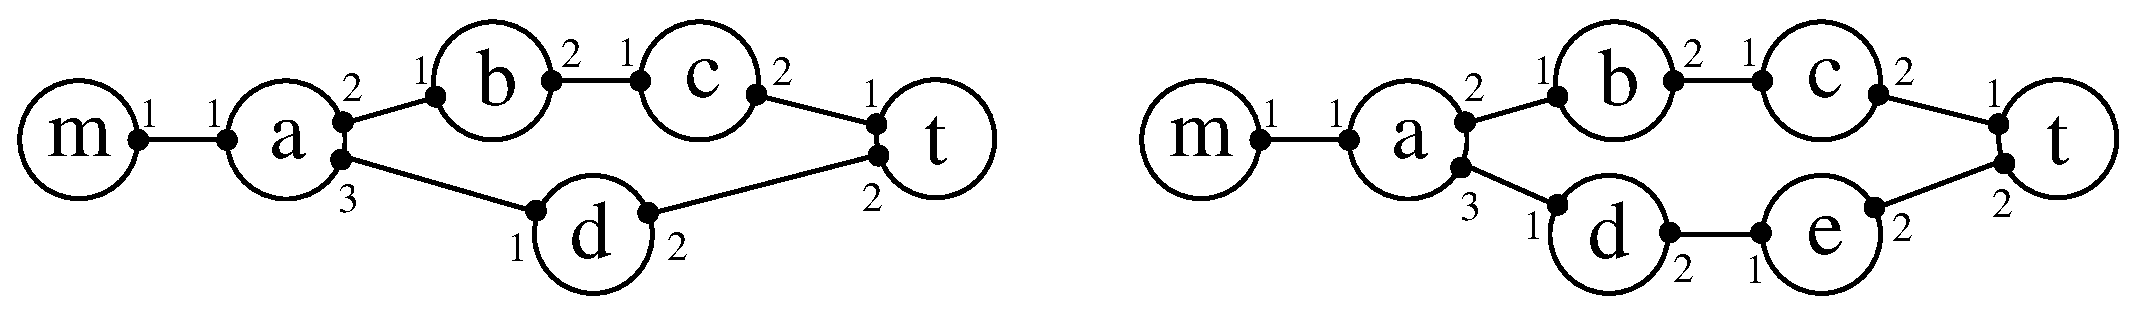
\includegraphics[scale=.24]{dyn.eps}
\caption{
Left: a case where routes between $m$ and $t$ have have different lengths, leading to the observation of fake neighbors. Right: a case where routes all have the same length, in this case no fake neighbors is produced by \traceroute.
Numbers are identifiers of the different interfaces of a router, and we denote by $a_i$ the $i^{th}$ interface of router $a$.
}
\label{fig-dyn}
\end{figure}


For example, in Figure~\ref{fig-dyn} (left), there are different routes from monitor $m$ to target $t$. Then, conducting a \traceroute\ measurement from $m$ to $t$, it may happen that the second packet (TTL=2) takes the upper route, while the third one (TTL=3) takes the bottom route. In this case, the output of \traceroute\ is the route $m$--$a_1$--$b_1$--$t$, which produces the false link $b_1$--$t$.
Similarly, in the case of Figure~\ref{fig-dyn} (right), because of load-balancer $a$, if the route changes during a \traceroute\ measurement, it may produce route $m$--$a$--$b_1$--$e_1$--$t$, or route $m$--$a$--$d_1$--$c_1$--$t$, then delivering false link $b_1$--$e_1$ or $d_1$--$c_1$. The output of \traceroute\ is a mix of all possible routes.


Nevertheless, there is a big difference between the two configurations depicted on Figure~\ref{fig-dyn}. 
In the left configuration, routes have different lengths and fake neighbors appear (that is, false links involving the target). On the opposite, in the right configuration, routes have the same length and we observe the actual neighbors of the target. This is a general fact: changes in the routes followed by packets have no impact on observed neighbors of the target {\em as long as all routes have the same length}. This is due to the fact that, in such cases, even though \traceroute\ may mix the routes, every node will always appear at the same distance both from the monitor and from the target. In particular, nodes in penultimate position on a route are neighbors of $t$, which is our only concern in the present context.
Note that the possibility of distinguishing configurations producing fake neighbors takes advantage of the specificity of our approach, which concentrate on the last hop. It does not allow to avoid false links anywhere else along the routes.

%Indeed, in our context, we are only concerned with the appearance of what we call \emph{fake neighbors}, that is, false links involving our target. To this regard, changes in the routes followed by packets have no impact {\em as long as they have the same length}.
%As showed above, if the lengths of the routes are different (Figure~\ref{fig-dyn}, left), the distance slices from the target, as they appear in \traceroute\ outputs, may change and lead to the observation of erroneous neighbors, $b_1$ in this case. But, on the opposite, if the lengths of the different routes are the same, then \traceroute\ may mix the routes but will always respect the distance slices from the targets. That is, all nodes along the routes will always appear at the same distance both from the source and the target in any \traceroute\ output. Consequently, every node involved in the last hop of a traceroute is a neighbor of $t$.

Then, our method to detect pairs $m,t$ likely to produce fake neighbors is to send several probes and examine the length of produced routes.
This raises the question of bounding the probability that there exist routes of different lengths that we did not detect, depending on the number of probes we sent. 
We did not address the question in its whole generality. Nevertheless, it is worth studying the case where there are exactly two routes of lengths $l_1$ and $l_2$ with $l_1<l_2$, having equal probability to be followed by \traceroute\ packets.
When a packet with TTL=$l_1$ is sent to target $t$, it follows one of the two routes. If it follows the shortest one, it arrives to $t$ and the route of length $l_1$ is discovered. If the packet follows the longest route, it does not reach $t$ and \traceroute\ outputs a route of length greater than $l_1$. It follows that the probability that $n$ probes give only routes of the same length is bounded by $2\times(1/2)^n$. In this case at least, it decreases exponentially with the number of probes, and only few probes should be necessary in order to detect the existence of two different route lengths.


%When sending to target $t$ a packet with TTL=$l_1$, it may either (i) reach $t$, thus leading to the discovery of the route of length $l_1$, or (ii) reach the node at distance $l_1$ on the other route, thus leading to the discovery of a longer route. It follows that the probability to have missed the longer route after $n$ \traceroute\ is $(1/2)^n$. In this particular case at least, it decreases exponentially with the number of probes, and only few probes should be necessary in order to detect the existence of the two routes.







%%%%%%%%%%%%%%%%%%%%%%%%%%%%%%%%%%%%%%%%%%%%%%%%%%%%%%%%%%%%%%%
%%%%%%%%%%%%%%%%%%%%%%%%%%%%%%%%%%%%%%%%%%%%%%%%%%%%%%%%%%%%%%%
\section{Sample measurement}\label{sec-measurement}
%%%%%%%%%%%%%%%%%%%%%%%%%%%%%%%%%%%%%%%%%%%%%%%%%%%%%%%%%%%%%%%
%%%%%%%%%%%%%%%%%%%%%%%%%%%%%%%%%%%%%%%%%%%%%%%%%%%%%%%%%%%%%%%


In this section, we show how to implement our method and we give the result of a measurement conducted on a random set of targets. This \emph{must not} been considered as an estimation of the degree distribution of any set of routers of internet. Indeed, as we mentioned previously, we did not implement any anti-aliasing technique nor any selection method for routers in the core of internet. These issues are key perspective and we let them for future work. The goal of this section is to demonstrate the practical effectiveness of our method and to show how we can clean obtained data without loosing information.



%%%%%%%%%%%%%%%%%%%%%%%%%%%%%%%%%%%%%%%%%%%%%%%%%%%%%%
\subsection{Measurement setup}\label{sec-setup}
%%%%%%%%%%%%%%%%%%%%%%%%%%%%%%%%%%%%%%%%%%%%%%%%%%%%%%

As we already mentioned, we used PlanetLab nodes as monitors for our measurement. Although these machines may not be uniformly distributed in the internet, we will assume that they are dispersed enough for our purpose.
One may argue that this is not the case because planetlab nodes lies mainly on academic networks. But still, destinations we choose are not on such networks and these networks have many connections to others all over the world. As shown by simulations, the critical point of comparison is between this number of outgoing connections and the degree of target routers.
Nevertheless, clearly, widening the set of monitors we use by integrating other sets, more widely distributed or larger, is one of our main perspectives, see Section~\ref{sec-discussion}.

Notice that some PlanetLab monitors may not be suitable for our needs. For instance, they may experience frequent shutdowns, or have poor internet connectivity. They may even filter \icmp\ (or belong to a network which does so). As managing these issues {\em before} the measurement is very difficult and subject to errors, we used {\em all} the monitors during our measurement, and discarded those which provided irrelevant data afterwards.


% Preliminary measurements showed that ~4.1% of non trivial random IPs answer to ICMP ECHO REQUEST. To get 10000 random IP answering ICMP ECHO REQUEST, we thus have to probe 1/0.041 x 10000 = ~250000 random IPs.
To construct our list of targets, we randomly sampled 250\,000 distinct 32 bit integers (IP-adresses), and sent an \icmp\ \echo\ \request\ to each of them. We recorded the 10\,000 first addresses which answered to this request. Again, note that our selected target are not necessarily in the core of the internet. This does not matter as we do not intend to get an estimation of the degree distribution, but we are only interested in illustrating our method.



Finally, we ran our measurement from the $5^{th}$ to the $6^{th}$ of July 2009 as follows. 
For each monitor, we shuffled the target list, obtained a few hours before, and generated a shell script
that sends a traceroute every second to each of the
targets, in the given shuffled order. This loop is repeated 10 times by each monitor, following its own shuffled order.
Once all the scripts have been generated, we sent each of them to the
corresponding monitor. Then, we sent a start command to every
monitor.
The measurement ended about 30 hours later, once 90\% monitors that had successfully received
\emph{and} started the script had terminated (some never terminate, mostly due to
shutdowns or errors unrelated to the script itself).
The raw output was then retrieved and analyzed locally.



%%%%%%%%%%%%%%%%%%%%%%%%%%%%%%%%%%%%%%%%%%%%%%%%%%%%%%
\subsection{Irrelevant monitors and targets}\label{sec-monitors-targets}
%%%%%%%%%%%%%%%%%%%%%%%%%%%%%%%%%%%%%%%%%%%%%%%%%%%%%%



The first step of our filtering process, which aims at obtaining reliable (and complete) data, consists in discarding monitors and targets that have irrelevant behavior with regard to our goal.



We say that a traceroute is {\em valid} if it reaches its target. As our targets are supposed to answer to \icmp\ \echo\ \request, and as we use \icmp\ \traceroute, all traceroutes should in principle be valid. However, it may happen that the monitor is unable to conduct the measurement (for instance if it has no \icmp\ capabilities) and, more importantly, a target may be unreachable at some time during the measurement.
In our case, we obtained 36\,928\,702 valid traceroutes from 544 monitors to 10\,000 targets (not all monitors and targets produce the same number of valid traceroutes) and examined their repartition among monitors and targets.

\begin{figure}[!ht]
\centering
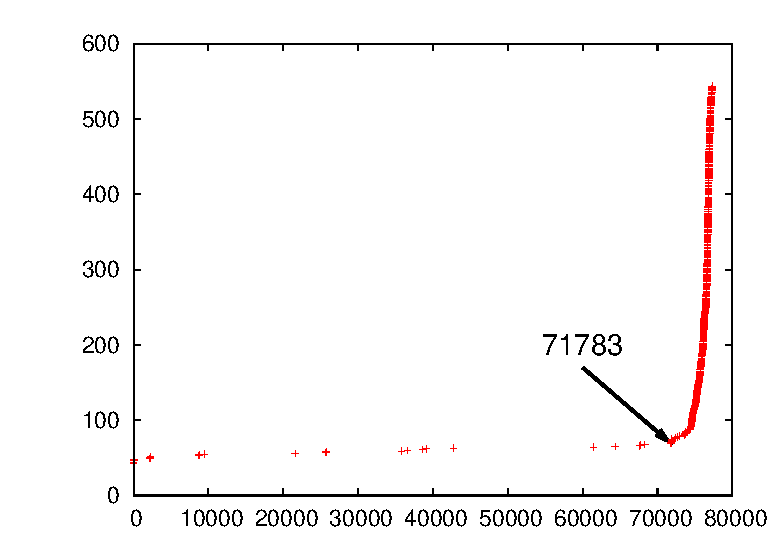
\includegraphics[scale=.5]{sources.valid.eps}
\caption{
Cumulative distribution of the number of valid traceroutes per monitor.
}
\label{fig-valid-monitor}
\end{figure}

Monitors from which we obtain a low number of valid traceroutes should be discarded. First because they make the number of monitors used in our inference larger than it actually is, and because they may parasite the following of the filtering process. The distribution of the number of valid traceroutes for each monitor (Figure~\ref{fig-valid-monitor}) shows that only 68 monitors out of 544 ($\sim$12\%) obtained less than 71\,783 valid traceroutes out of 77\,316 ($\sim$92\%), which is the maximum number of valid traceroutes collected by a monitor. We then discarded these 68 monitors and kept only the data from the remaining 476 for the following. According to Section~\ref{sec-simulations}, this should not make us loose any data.


\begin{figure}[!ht]
\centering
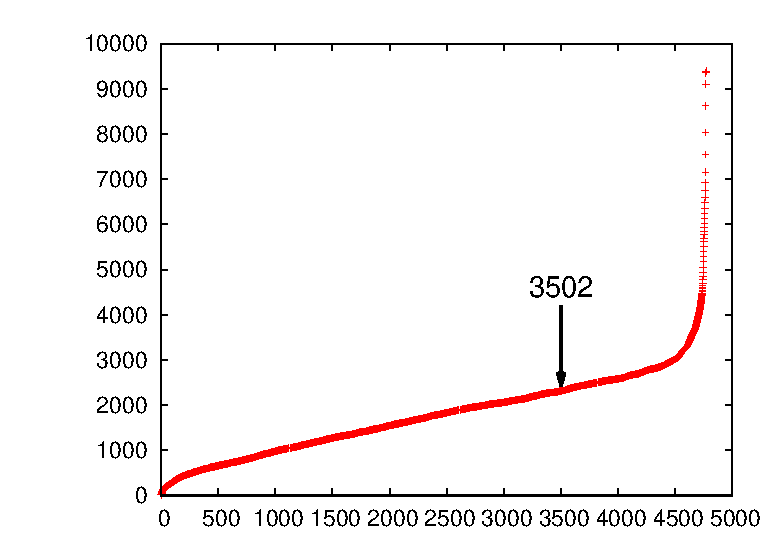
\includegraphics[scale=.5]{targets.valid.eps}
\caption{
Cumulative distribution of the number of valid traceroutes per target. A point with coordinates ($x$, $y$) means that exactly $y$ monitors (resp. targets) obtained $x$ valid traceroutes or less.
}
\label{fig-valid-target}
\end{figure}

Similarly, targets for which we obtain no valid traceroute, or only few, should be discarded: we have too limited information on them. This is probably due to target shutdowns or network failures. We will assume that there is no correlation between this and the target degree. We first removed the 605 targets obtaining no valid traceroute (this may be due to the fact that the target are no longer connected at the time of the measurement), and we plotted the distribution of the number of valid traceroutes per target (Figure~\ref{fig-valid-target}). It shows that 2314 targets out of 9395 remaining ones ($\sim$25\%) obtained less than 3502 valid traceroutes out of 4760 ($\sim$74\%). In the sequel, we do not consider them anymore and we go on with the 7081 remaining targets. Note that, necessarily, these remaining targets have been observed by at least 350 different monitors (since a monitor produces at most 10 valid traceroutes per destination).





%%%%%%%%%%%%%%%%%%%%%%%%%%%%%%%%%%%%%%%%%%%%%%%%%%%%%%
\subsection{Fake neighbors correction}
%%%%%%%%%%%%%%%%%%%%%%%%%%%%%%%%%%%%%%%%%%%%%%%%%%%%%%

At this point, only traceroutes from 476 monitors to 7\,081 targets remain. Thanks to the 10 repetitions of \traceroute\ between each pair of monitor and target, we can now filter the part of data that may contain erroneous neighbors. We showed in Section~\ref{sec-fake} that this mistrustful data comes from the pairs for which all valid traceroutes have different lengths. Fortunately, about 75\% of them produced constant-length routes. In order to remove the others from our data, we plotted the distribution of the number of monitors that produced all its traceroutes of the same length per target (see Figure~\ref{fig-routelength}). It turns out that only 980 targets out of 7\,081 ($\sim$14\%) have less than 350 monitors producing constant-length routes.
Then, we discarded all mistrustful pairs and kept only the 6\,101 targets still observed by enough monitors afterwards. Again, we make the assumption that having routes of different lengths is independent from target degree.



\begin{figure}[!ht]
\centering
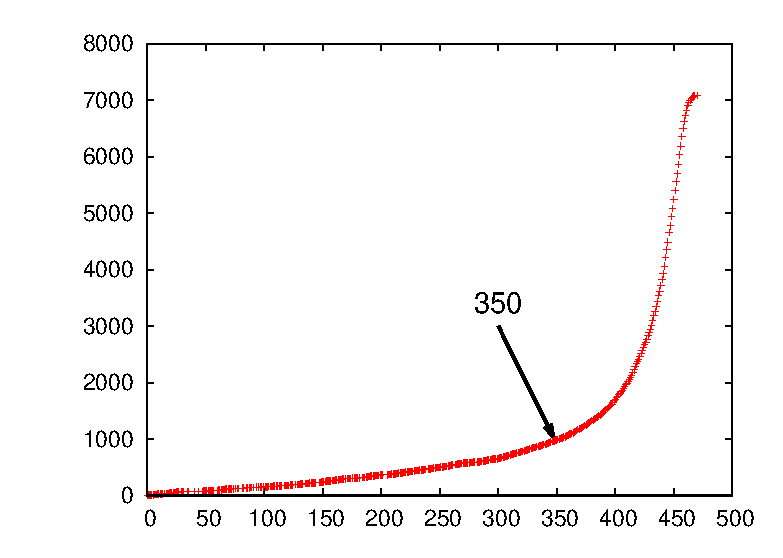
\includegraphics[scale=.5]{routelength.eps}
\caption{
Cumulative distribution of the number of targets per monitor reached by constant-length routes. A point with coordinate ($x$, $y$) means that exactly $y$ targets obtained all traceroutes with the same length from $x$ monitors or less.
}
\label{fig-routelength}
\end{figure}

%%%%%%%%%%%%%%%%%%%%%%%%%%%%%%%%%%%%%%%%%%%%%%%%%%%%%%
\subsection{Results}
%%%%%%%%%%%%%%%%%%%%%%%%%%%%%%%%%%%%%%%%%%%%%%%%%%%%%%

The distribution of the number of neighbor interfaces\footnote{Traceroutes producing a star in last but one position do not give any neighbor interface of the target in the considered topology, and therefore do not contribute to the distribution.}
observed for each target in our sample measurement is given in Figure~\ref{fig-degrees}. Let us insist on the fact that this is {\em not} an estimation of any degree distribution: neighbor routers may be counted several times as we do not recognize different interfaces of a same router, and the sample contains targets in the {\em border} of the topology (for which we miss some neighbors).

\begin{figure}[!ht]
\centering
\includegraphics[scale=.5]{constant-length.distrib.eps}
\caption{
Final distribution of the number of neighboring interfaces per target.
}
\label{fig-degrees}
\end{figure}

Notice however that most targets have a low number of neighbor interfaces, which is in accordance with domain knowledge, but that none of them has a very high degree. Indeed, although our method would underestimate the degrees of such nodes, simulations show that their order of magnitude would not change. But the largest value observed in our measurement is 57, which is itself an upper bound of the number of neighbor routers (remind that several interfaces may belong to a same router). This means that there was no high-degree node in our random sample of 10\,000 nodes, and that such nodes are therefore very rare (much rarer than expected in a power-law distribution). As a consequence, our method is appropriate for observation of the vast majority of nodes.

%%%%%%%%%%%%%%%%%%%%%%%%%%%%%%%%%%%%%%%%%%%%%%%%%%%%%%%%%%%%%%%
%%%%%%%%%%%%%%%%%%%%%%%%%%%%%%%%%%%%%%%%%%%%%%%%%%%%%%%%%%%%%%%
\section{Conclusion and perspectives.}\label{sec-result}\label{sec-discussion}
%%%%%%%%%%%%%%%%%%%%%%%%%%%%%%%%%%%%%%%%%%%%%%%%%%%%%%%%%%%%%%%
%%%%%%%%%%%%%%%%%%%%%%%%%%%%%%%%%%%%%%%%%%%%%%%%%%%%%%%%%%%%%%%

We presented a method to obtain an interface of each neighbor of a router in the core of the internet. This constitutes an important step towards precise estimation of the degree distribution of the IP-level router topology, which is our main perspective. It now relies on anti-aliasing techniques, thus increasing significantly the importance of this problem, and on selection of targets from which to infer the global degree distribution. Indeed, randomly selecting interfaces does not lead to random {\em routers} selection as the sampling is biased by the number of interfaces attached to routers. Correction of this bias is necessary.

Our work also raises several key questions which may be tackled formally. In particular, one may formally establish the results we obtain here with simulations, such as the fact that our approach succeeds in discovering all neighbors of targets, or the limited impact of the size of the underlying graph, which we empirically observe here.
One may also conduct simulations and formal analysis on other kinds of graphs, in particular scale-free graphs and HOT models. We are currently exploring these directions.

Another direction for improving our results is to increase the number of involved monitors, in order to obtain more reliable measurements for high-degree nodes (we have seen that this would not improve results for low-degree nodes). To that purpose, one may use {\em looking glasses}, \ie\ websites providing the possibility to run \traceroute\ measurements from them (more than one thousand such sites are currently available), as well as monitors from the \emph{DIMES project}, which counts approximately one thousand machines. Notice that these monitors and those of PlanetLab may be used all together, and that their number increases rapidly.

%Our work may also help in searching for very high degree nodes in the IP-level topology, and testing their existence. As such nodes are quite rare (there was no such node in our random sample of targets), one has to setup a method to track them. For instance, one may focus on nodes which appear frequently on large traceroute measurements from many monitors to many targets (classical measurements).

%Finally, as our work is dedicated to the {\em core} of the topology, we argue for the need of methods dedicated to its {\em boerder} in order to obtain a global view of the topology. The design of two complementary measurement methods is motivated by the fundamentally different nature of these two parts of the internet \cite{willinger}.

%\section{Conclusion.}
%\label{sec-conclusion}
%\medskip
%\noindent
%{\bf Acknowledgements.}
%...

{%\small
%\scriptsize
\bibliographystyle{./IEEEtran}
%\bibliographystyle{plain}
%\bibliographystyle{abbrv}
\bibliography{biblio}
}


\end{document}


\newpage
\begin{appendix}



%%%%%%%%%%%%%%%%%%%%%%%%%%%%%%%%%%%%%%%%%%%%%%%%%%%%%%%%%%%%%%%
\section{More simulation results}\label{ap-simul}
%%%%%%%%%%%%%%%%%%%%%%%%%%%%%%%%%%%%%%%%%%%%%%%%%%%%%%%%%%%%%%%


\begin{figure}[!ht]
\centering
\includegraphics[angle=-90,scale=.23]{poisson_5_1M.ps}
\includegraphics[angle=-90,scale=.23]{erdos_5_10M.ps}
\caption{
Degree distributions observed in our simulations on Poisson graphs with average degree $5$. Left: one million nodes. Right: ten million nodes. In both cases, we plot the true degree distribution (full) and the ones observed with $25$, $100$, $200$ and $500$ monitors.
}
\label{fig-simul2}
\end{figure}



\begin{figure}[!ht]
\centering
\includegraphics[angle=-90,scale=.23]{poisson_10_1M.ps}
\includegraphics[angle=-90,scale=.23]{erdos_10_10M.ps}
\caption{
Degree distributions observed in our simulations on Poisson graphs with average degree $10$. Left: one million nodes. Right: ten million nodes. In both cases, we plot the true degree distribution (full) and the ones observed with $25$, $100$, $200$ and $500$ monitors.
}
\label{fig-simul3}
\end{figure}


%%%%%%%%%%%%%%%%%%%%%%%%%%%%%%%%%%%%%%%%%%%%%%%%%%%%%%%%%%%%%%%
\section{Paramaters used in the measurement process}\label{ap-param}
%%%%%%%%%%%%%%%%%%%%%%%%%%%%%%%%%%%%%%%%%%%%%%%%%%%%%%%%%%%%%%%


We give below \traceroute\ parameters and ssh/scp parameters used in our measurement.

\medskip
\noindent \traceroute\ parameters:
\begin{itemize}
\item Protocol: ICMP
\item  Number of probes sent per TTL: 1
\item  Minimum time between 2 traceroutes: 1s
\item  Address-to-name lookup: No
\item  Minimum time between 2 probes: 0
\item  Other parameters use default values.
\end{itemize}

\medskip
\noindent ssh/scp parameters:
\begin{itemize}
\item  Connect timeout: 600s
\item  Use compression: yes
\item  Kill after timeout expires: yes
\end{itemize}


\end{appendix}



